% =========================================================================
%  Presentación del proyecto
%  Tema: Modelo fluido TCP/RED de Misra-Gomez-Towsley
%  Autor: Abel Santiago García Ortiz
% =========================================================================
\documentclass[10pt,aspectratio=169]{beamer}

\usetheme{metropolis}
\usepackage[utf8]{inputenc}
\usepackage[T1]{fontenc}
\usepackage[spanish,es-nodecimaldot]{babel}
\usepackage{amsmath,amssymb}
\usepackage{graphicx}
\usepackage{booktabs}
\usepackage{xcolor}
\usepackage{tikz}
\usepackage{hyperref}

% Colores del tema (paleta metropolis modificada suavemente)
\definecolor{tcpblue}{HTML}{1F77B4}
\definecolor{redred}{HTML}{D62728}
\definecolor{abmgreen}{HTML}{2CA02C}

% Metadatos
\title{Modelo fluido TCP/RED}
\subtitle{Aproximación numérica, análisis de estabilidad y bifurcación de Hopf}
\author{Abel Santiago García Ortiz}
\institute{UPB, 2026}
\date{\small Modelamiento Matemático}

% =========================================================================
\begin{document}

% --------- SLIDE 1: PORTADA ----------------------------------------------
\maketitle

% --------- SLIDE 2: EL GANCHO --------------------------------------------
\begin{frame}{¿Cuándo Internet oscila?}

\begin{columns}[T,onlytextwidth]
\column{0.55\textwidth}
Cuando descargas un archivo, ves un video o haces una videollamada,
dos algoritmos invisibles están negociando:

\vspace{0.4em}
\begin{itemize}
\item Tu computador (TCP) decide cuántos paquetes enviar.
\item El router decide cuándo descartar paquetes para
      pedirte que bajes el ritmo.
\end{itemize}

\vspace{0.5em}
\textbf{El problema:} este lazo puede volverse inestable y hacer
que miles de conexiones oscilen sincronizadamente.

\column{0.45\textwidth}
\centering
\begin{tikzpicture}[scale=0.85]
\node[draw,rounded corners,fill=tcpblue!20,minimum width=2.6cm,minimum height=0.8cm] (tcp) at (0,2) {Fuentes TCP};
\node[draw,rounded corners,fill=redred!20,minimum width=2.6cm,minimum height=0.8cm] (red) at (0,0) {Router con RED};
\draw[->,thick] (tcp.east) to[bend left=45] node[right,font=\small]{paquetes} (red.east);
\draw[->,thick] (red.west) to[bend left=45] node[left,font=\small]{descartes} (tcp.west);
\node[font=\small,gray] at (0,1) {lazo cerrado};
\end{tikzpicture}
\end{columns}

\vspace{1.5em}
\centering
\small\text{Objetivo del proyecto: modelar, simular y entender ese fenómeno.}
\end{frame}

% --------- SLIDE 3: LAS TRES VARIABLES -----------------------------------
\begin{frame}{El sistema: tres variables}

\begin{columns}[T,onlytextwidth]
\column{0.33\textwidth}
\centering
\textbf{\color{tcpblue}$W(t)$}\\[0.3em]
\textit{Ventana TCP}\\[0.5em]
\small Cuántos paquetes puede enviar cada fuente sin esperar confirmación.

\vspace{0.5em}
{\footnotesize Aumenta gradualmente, baja a la mitad cuando hay pérdida.}

\column{0.33\textwidth}
\centering
\textbf{\color{redred}$q(t)$}\\[0.3em]
\textit{Cola del router}\\[0.5em]
\small Cuántos paquetes están haciendo fila esperando ser transmitidos.

\vspace{0.5em}
{\footnotesize Sube si llegan más rápido de los que salen, baja si no.}

\column{0.33\textwidth}
\centering
\textbf{\color{abmgreen}$x(t)$}\\[0.3em]
\textit{Cola promedio (EWMA)}\\[0.5em]
\small Versión \emph{suavizada} de $q$ que el algoritmo RED usa para decidir.

\vspace{0.5em}
{\footnotesize Sigue a $q$ con un retraso controlado por $w_q$.}
\end{columns}

\vspace{1em}
\centering
Estas tres variables interactúan y dan lugar a toda la dinámica.
\end{frame}

% --------- SLIDE 4: LAS ECUACIONES ---------------------------------------
\begin{frame}{Modelado matemático: tres EDOs acopladas}

\textbf{Modelo de Misra-Gomez-Towsley} (SIGCOMM 2000):
\begin{align*}
\frac{dW}{dt} &= \underbrace{\frac{1}{R}}_{\text{sube }+1\text{/RTT}} - \underbrace{\frac{W^2}{2R}\, p(x)}_{\text{baja a la mitad si hay pérdida}}\\[0.2em]
\frac{dq}{dt} &= \underbrace{-\,C}_{\text{salen a tasa }C} + \underbrace{\frac{NW}{R}}_{\text{entran }N\text{ flujos a tasa }W/R}\\[0.2em]
\frac{dx}{dt} &= \underbrace{w_q\, C\,(q-x)}_{\text{filtro paso-bajo: }x\to q\text{ con constante }1/w_qC}
\end{align*}

\vspace{0.3em}
\small
\textbf{Parámetros}: $N$ flujos, $C$ capacidad del enlace, $R$ tiempo de ida y vuelta (RTT),
$w_q$ peso del promediado RED.

\vspace{0.3em}
\textbf{Curva de descarte RED:} $p(x)$ es 0 hasta $q_{\min}$, lineal hasta $q_{\max}$, satura en $p_{\max}$.
\end{frame}

% --------- SLIDE 5: ¿POR QUÉ NO HAY SOLUCIÓN ANALÍTICA? -------------------
\begin{frame}{¿Por qué no podemos resolverlo a mano?}

Cuatro razones hacen imposible una fórmula cerrada para $W(t)$, $q(t)$, $x(t)$:

\vspace{0.5em}
\begin{enumerate}
\item \textbf{No linealidad:} el término $W^2 \cdot p$ es cuadrático en $W$.
\vspace{0.3em}
\item \textbf{Función por tramos:} $p(x)$ tiene esquinas en $q_{\min}$ y $q_{\max}$.
\vspace{0.3em}
\item \textbf{Acoplamiento:} $W \to q \to x \to p \to W$ no se separa por cambio de variable.
\vspace{0.3em}
\item \textbf{Retardo} en la versión completa: $W$ reacciona a $p$ con un RTT de atraso.
\end{enumerate}

\vspace{0.8em}
\centering
Por eso recurrimos a métodos numéricos.
\end{frame}

% --------- SLIDE 6: REDUCCIÓN Y EQUILIBRIO -------------------------------
\begin{frame}{Reducción a primer orden y equilibrio analítico}

\textbf{Buena noticia:} el sistema ya está en forma de primer orden.
\vspace{0.3em}

Vector de estado: $\mathbf{y} = (W, q, x)^\top \in \mathbb{R}^3$.\\
Función: $d\mathbf{y}/dt = \mathbf{f}(t, \mathbf{y})$.

\vspace{0.7em}
Imponiendo $\mathbf{f} = \mathbf{0}$ (sin cambios temporales) obtenemos
el punto donde el sistema descansaría:
\[
\boxed{\; W^* = \frac{R\,C}{N}, \qquad p^* = \frac{2N^2}{R^2 C^2}, \qquad q^* = q_{\min} + \frac{p^*}{p_{\max}}(q_{\max}-q_{\min}) \;}
\]

\vspace{0.5em}
Con los parámetros nominales:
\begin{center}
\begin{tabular}{lll}
$W^* = 15{,}375$ pkt & \quad $q^* = 196{,}53$ pkt & \quad $p^* = 0{,}85\%$
\end{tabular}
\end{center}

\vspace{0.6em}
\small
\textit{Sustituir $\mathbf{y}^*$ en $\mathbf{f}$ produce residual $\sim 10^{-15}$
(precisión de máquina): primera prueba de validación del código.}
\end{frame}

% --------- SLIDE 7: MÉTODOS NUMÉRICOS ------------------------------------
\begin{frame}{Tres métodos numéricos programados}

\centering
\small
\begin{tabular}{lccl}
\toprule
\textbf{Método} & \textbf{Orden} & \textbf{Evals.\ de $f$/paso} & \textbf{Rol en el proyecto} \\
\midrule
\textbf{\color{tcpblue}Euler explícito} & 1 & 1 & Referencia mínima \\[0.3em]
\textbf{\color{redred}Runge-Kutta 4 (RK4)} & 4 & 4 & Estándar de la industria \\[0.3em]
\textbf{\color{abmgreen}Adams-Bashforth-Moulton 4} & 4 & 2 & Multipaso eficiente \\
\bottomrule
\end{tabular}

\vspace{1em}
\begin{itemize}
\item Los tres están programados desde cero.
\item ABM4 = predictor explícito + corrector implícito (\textit{PECE}); arranca con RK4.
\item \textbf{Validación previa}: sobre el oscilador armónico (que sí tiene solución analítica)
los tres reproducen sus órdenes teóricos con pendientes $1{,}01$, $4{,}00$, $4{,}00$.
\end{itemize}
\end{frame}

% --------- SLIDE 8: VALIDACIÓN Y HERRAMIENTAS ----------------------------
\begin{frame}{Validación y herramientas}

\textbf{Referencia de comparación:} \texttt{scipy.integrate.solve\_ivp}
método RK45 (Dormand-Prince adaptativo) con tolerancias
$10^{-10}$ y $10^{-12}$.

\vspace{0.5em}
\textbf{Métricas:}
\begin{itemize}
\item Error global $\|\mathbf{e}\|_\infty$ por componente.
\item Pendiente empírica en escala log-log: ¿coincide con el orden teórico?
\item Número de evaluaciones de $\mathbf{f}$ (costo computacional).
\end{itemize}

\vspace{0.6em}
\textbf{Stack:} Python + NumPy + SciPy + Matplotlib.
\textbf{Animaciones:} \texttt{FuncAnimation} + ffmpeg.

\vspace{0.6em}
\textbf{Repositorio reproducible:}
\centering
\href{https://github.com/abel8000001/Proyecto-numerico}{\texttt{github.com/abel8000001/Proyecto-numerico}}
\end{frame}

% --------- SLIDE 9: RÉGIMEN ESTABLE -------------------------------------
\begin{frame}{Resultado 1: régimen estable}

\begin{columns}[T,onlytextwidth]
\column{0.55\textwidth}
\centering
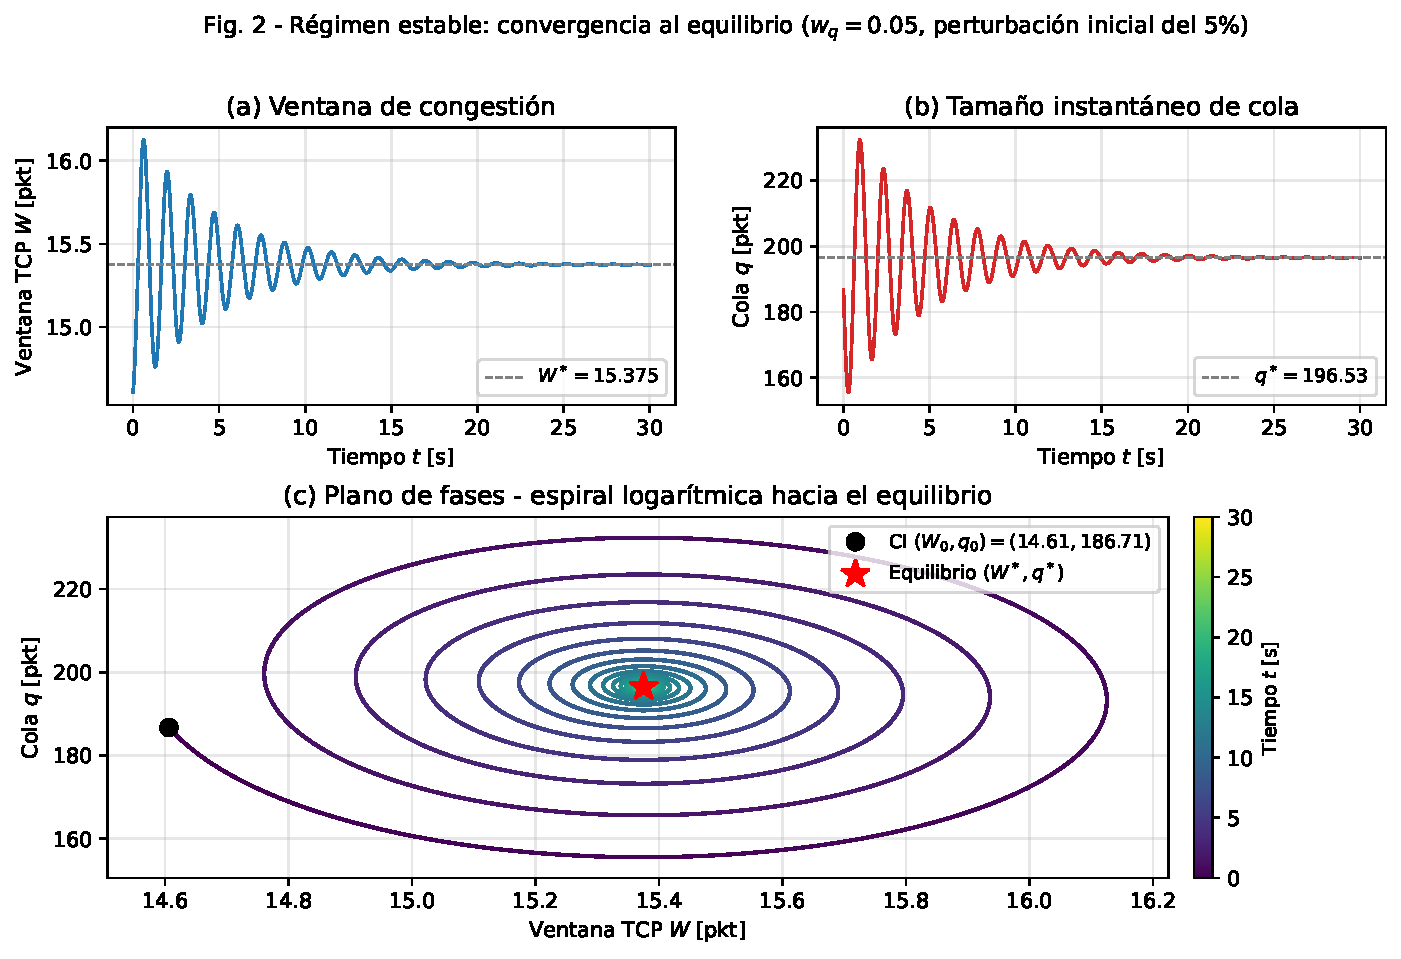
\includegraphics[width=\linewidth]{figs/fig2_stable.pdf}



\column{0.45\textwidth}
\textbf{Setup:} $w_q = 5\times 10^{-2}$, perturbación inicial del $5\%$, RK4, $h=10^{-3}$.

\vspace{0.5em}
\textbf{Resultado:}
\begin{itemize}
\item Convergencia exponencial al equilibrio.
\item Error vs.\ equilibrio analítico: \\
      \quad $0{,}010\%$ en $W$, $0{,}013\%$ en $q$.
\item Plano de fases: espiral logarítmica.
\item Período observado: $1{,}36$~s, idéntico al predicho por el análisis lineal.
\end{itemize}
\end{columns}
\end{frame}

% --------- SLIDE 10: CONVERGENCIA ----------------------------------------
\begin{frame}{Resultado 2: convergencia de los métodos}

\begin{columns}[T,onlytextwidth]
\column{0.6\textwidth}
\centering
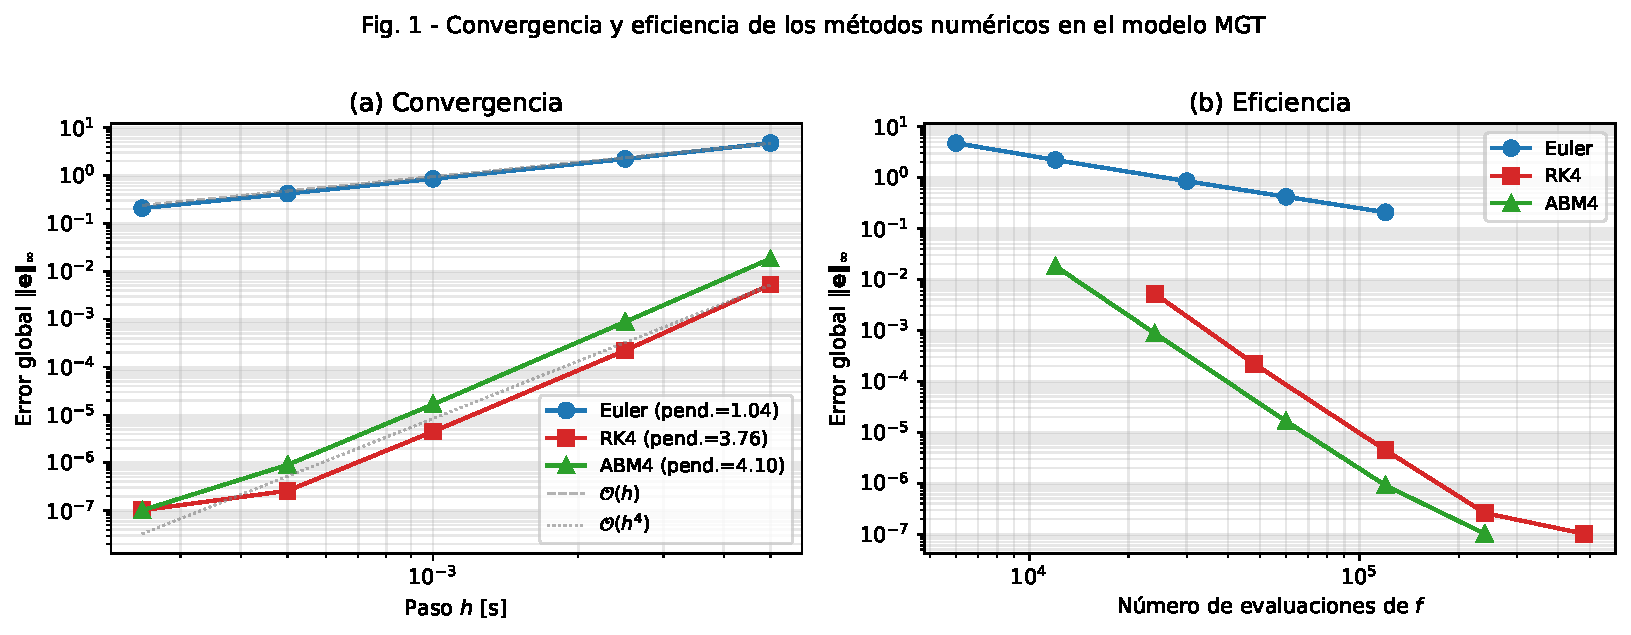
\includegraphics[width=\linewidth]{figs/fig1_convergence.pdf}

\column{0.01\textwidth}

\column{0.4\textwidth}
\textbf{Pendientes empíricas:}
\begin{itemize}
\item \textcolor{tcpblue}{Euler}: $1{,}04$ (teórico: 1) \checkmark
\item \textcolor{redred}{RK4}: $3{,}76$ (teórico: 4) \checkmark
\item \textcolor{abmgreen}{ABM4}: $4{,}10$ (teórico: 4) \checkmark
\end{itemize}

\vspace{0.6em}
\textbf{Observación clave:}\\
Los tres métodos confirman su orden teórico sobre el modelo MGT.

\vspace{0.5em}
{\small RK4 se aplana en $h$ pequeño porque su error se acerca al de la referencia.}
\end{columns}
\end{frame}


% --------- SLIDE 11: HOPF — INTRO ----------------------------------------
\begin{frame}{Resultado 3: ¿qué pasa si cambiamos $w_q$?}

\textbf{Recordatorio:} $w_q$ controla qué tan rápido el promedio $x$ sigue a la cola real $q$.

\vspace{0.6em}
\textbf{Pregunta natural:} ¿qué ocurre si $w_q$ es pequeño? \\
Físicamente: el router promedia más lentamente, 
introduce un retardo efectivo en el lazo.

\vspace{0.8em}
\textbf{Bifurcación de Hopf:} cuando un parámetro cruza un valor crítico, un equilibrio estable
pierde su estabilidad y aparece un ciclo límite (oscilación sostenida).

\vspace{0.6em}
\textbf{Detección numérica:}
\begin{enumerate}
\item Calcular el jacobiano $J = \partial \mathbf{f}/\partial \mathbf{y}$ en el equilibrio.
\item Sus autovalores indican la estabilidad de cada modo:
\begin{itemize}
\item parte real negativa $\Rightarrow$ modo decae (estable),
\item parte real positiva $\Rightarrow$ modo crece (inestable),
\item parte imaginaria $\Rightarrow$ oscilación.
\end{itemize}
\item Bisección hasta encontrar $w_q^c$ donde la parte real cruza cero.
\end{enumerate}
\end{frame}

% --------- SLIDE 12: HOPF — RESULTADOS -----------------------------------
\begin{frame}{Resultado 3: bifurcación de Hopf supercrítica}

\begin{columns}[T,onlytextwidth]
\column{0.55\textwidth}
\centering
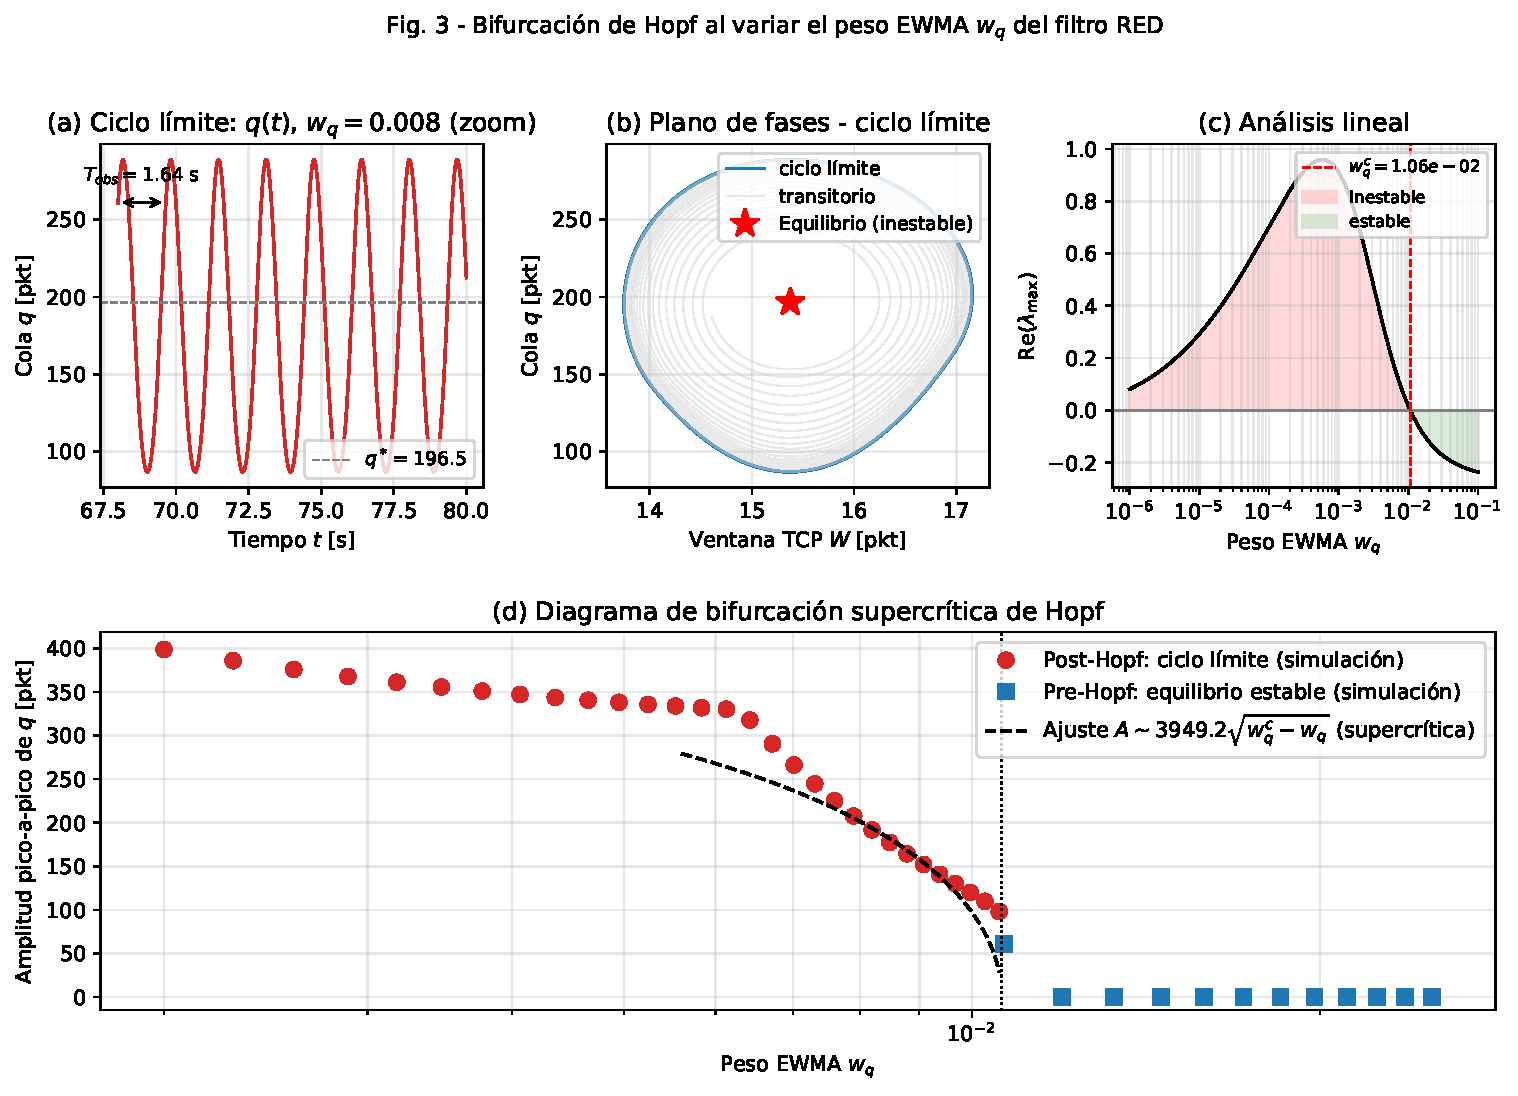
\includegraphics[width=\linewidth]{figs/fig3_hopf.pdf}

\column{0.01\textwidth}

\column{0.45\textwidth}
\begin{itemize}
\item \textbf{Hallazgo:} en $w_q^c = 1{,}06 \times 10^{-2}$, par complejo $\pm 4{,}586j$ cruza el eje imaginario.\\
\item \textbf{Predicción del análisis lineal:} ciclo límite con período $T_c = 1{,}37$~s.\\
\item \textbf{Observado en simulación} (a $w_q = 8\times 10^{-3}$, post-Hopf): $T_\text{obs} = 1{,}64$~s.
\end{itemize}

\end{columns}
\end{frame}

% --------- SLIDE 13: HOPF — LEY UNIVERSAL --------------------------------
\begin{frame}{El diagrama de bifurcación confirma la ley universal}

\begin{columns}[T,onlytextwidth,c]
\column{0.55\textwidth}
\centering
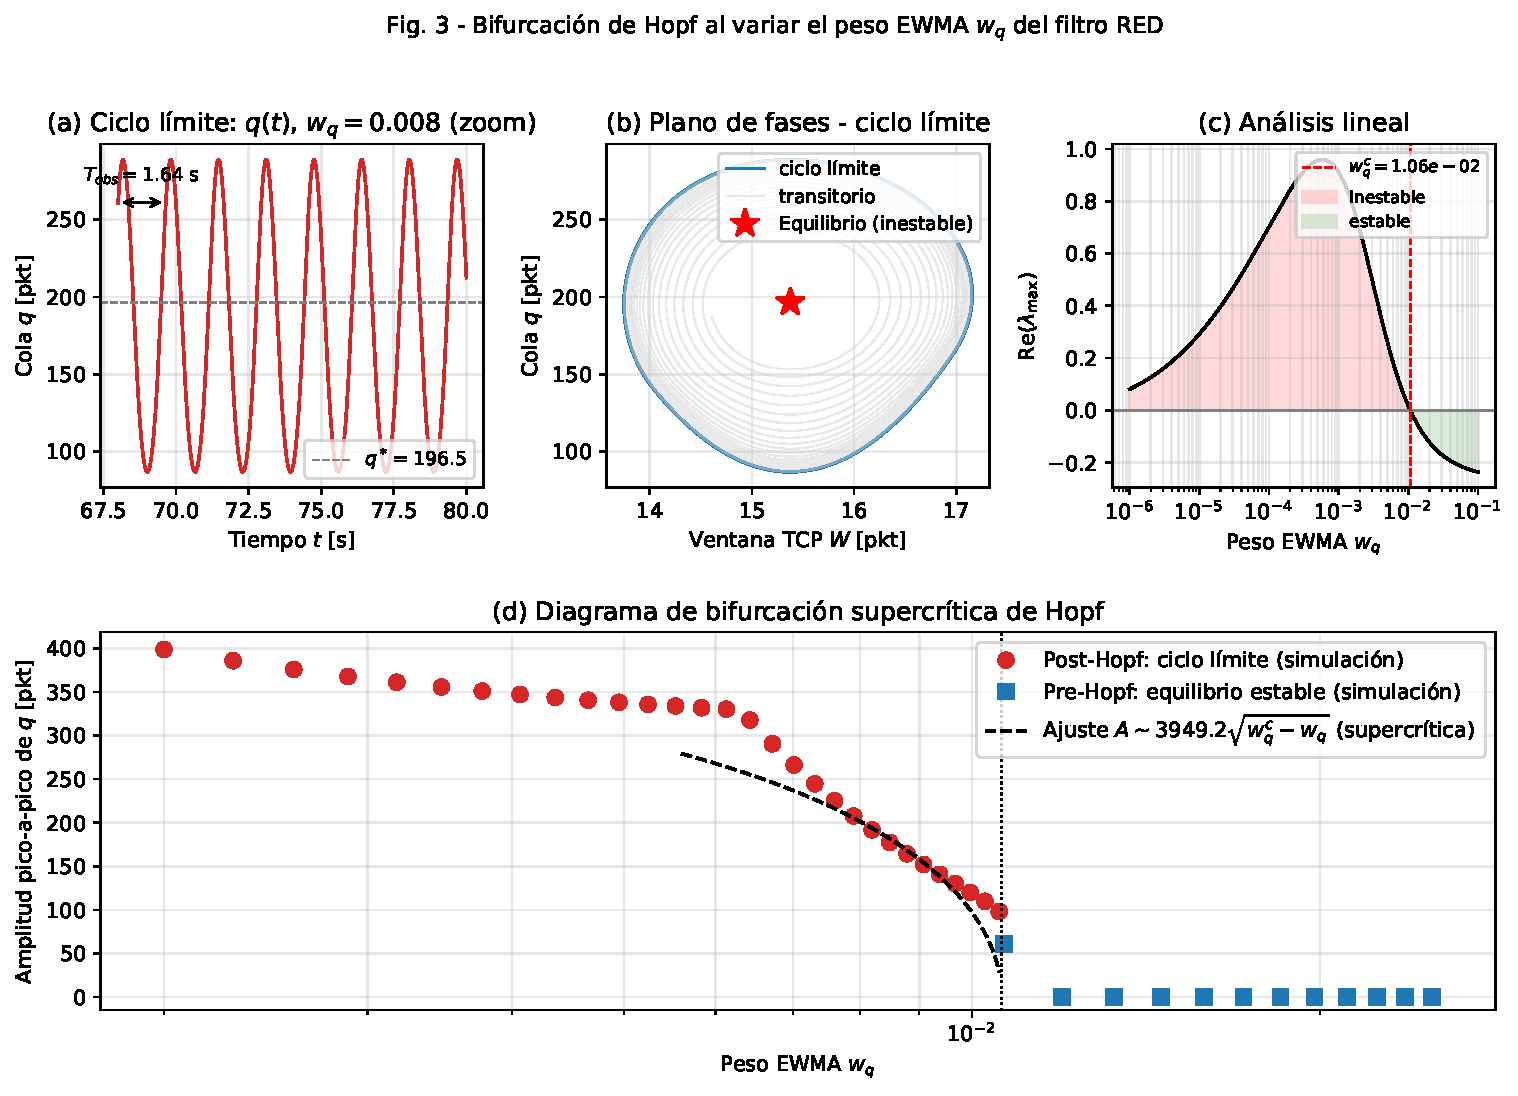
\includegraphics[width=\linewidth]{figs/fig3_hopf.pdf}

\column{0.01\textwidth}

\column{0.45\textwidth}
\vspace{0.5em}

Panel (d): para cada $w_q$ medimos la amplitud pico--pico de $q$ en el atractor.

\vspace{0.5em}
\textbf{Cerca de $w_q^c$}, los puntos siguen:
\[
A \approx 3949\sqrt{w_q^c - w_q}
\]

Esta dependencia de raíz cuadrada es la ley universal de la Hopf supercrítica
(viene de la forma normal del sistema).

\vspace{0.5em}
La verificación numérica confirma que la bifurcación es supercrítica, ya que los ciclos
se mantienen constantes

\vspace{0.5em}
{\small Lejos del punto crítico la curva se aplana: el ciclo toca $q=0$ y la saturación física limita la amplitud.}
\end{columns}
\end{frame}

% --------- SLIDE 14: ANIMACIÓN -------------------------------------------
\begin{frame}{Animación: la transición en vivo}

\begin{columns}[T,onlytextwidth]
\column{0.55\textwidth}
\centering
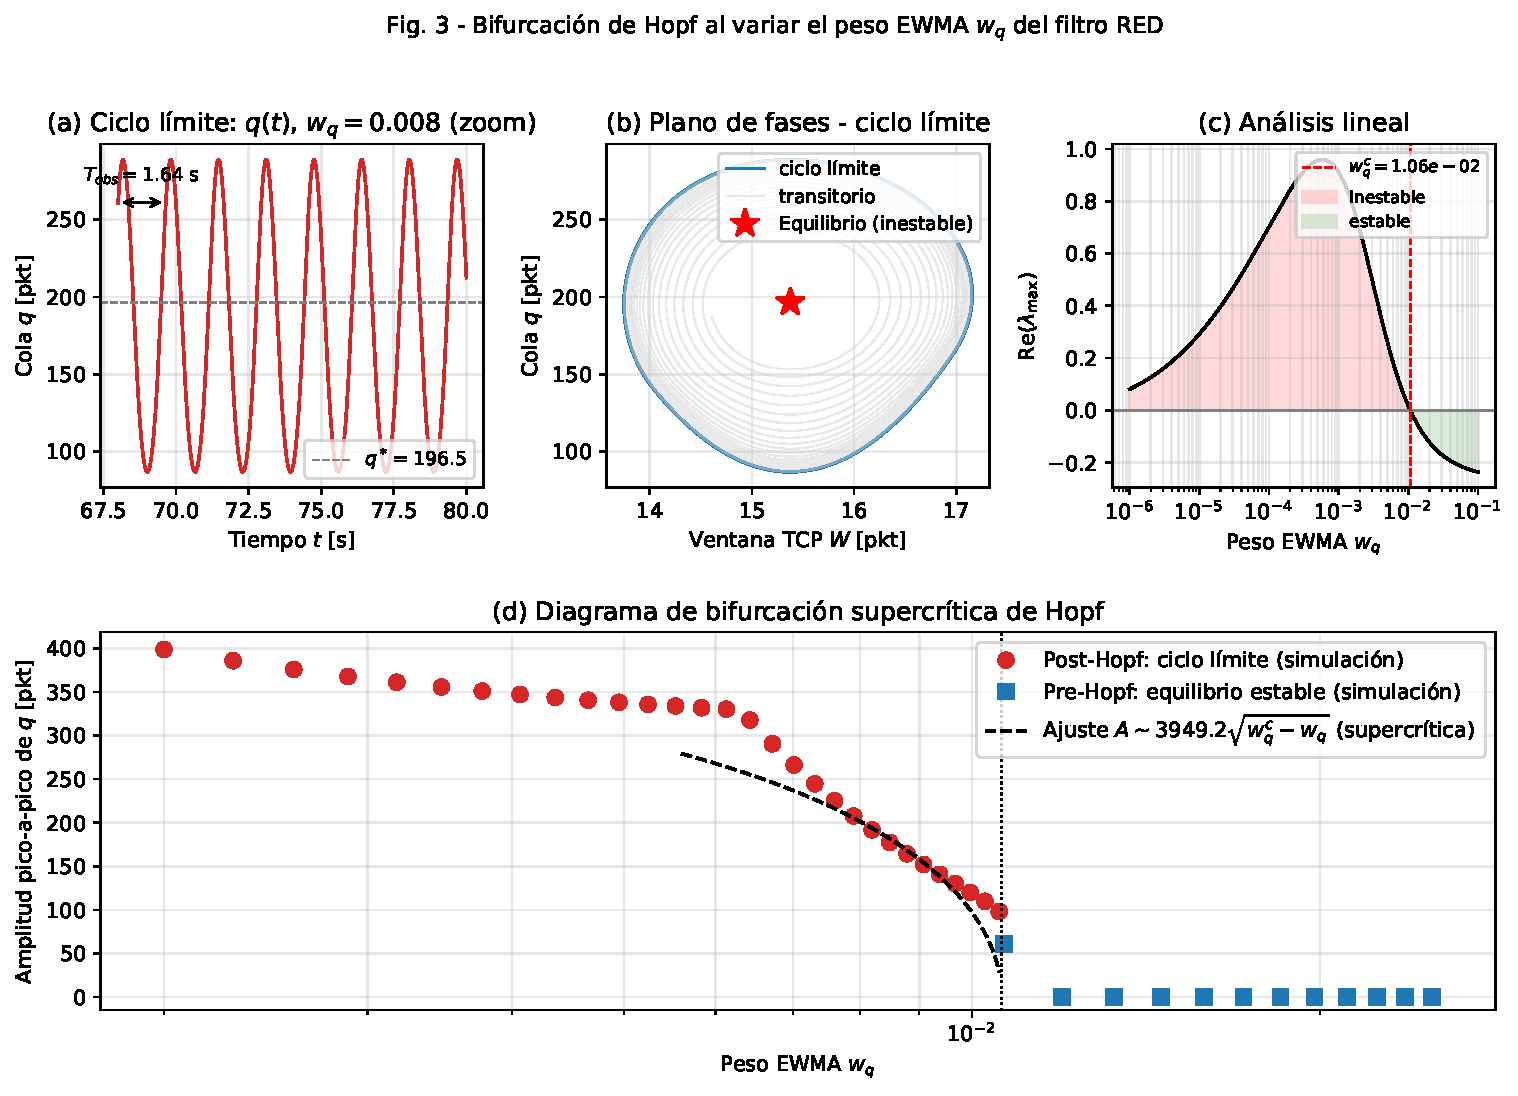
\includegraphics[width=\linewidth]{figs/fig3_hopf.pdf}

\column{0.01\textwidth}

\column{0.45\textwidth}
La transición estable a ciclo límite al cambiar $w_q$ se ve
mejor en movimiento:

\vspace{0.6em}
\textbf{Animación 1:}
\begin{itemize}
\item Fase 1: $w_q$ grande $\to$ espiral hacia el equilibrio.
\item Fase 2: $w_q$ pequeño $\to$ ciclo límite cerrado.
\end{itemize}

\vspace{0.7em}
\textbf{Ver online:}\\[0.3em]
\url{https://youtu.be/pxrYpyrs_wQ}

\end{columns}
\end{frame}

% --------- SLIDE 15: TRABAJO FUTURO - DOS RUTAS --------------------------
\begin{frame}{Trabajo adicional: extensión a dos rutas paralelas}

\begin{columns}[T,onlytextwidth]
\column{0.55\textwidth}
\centering
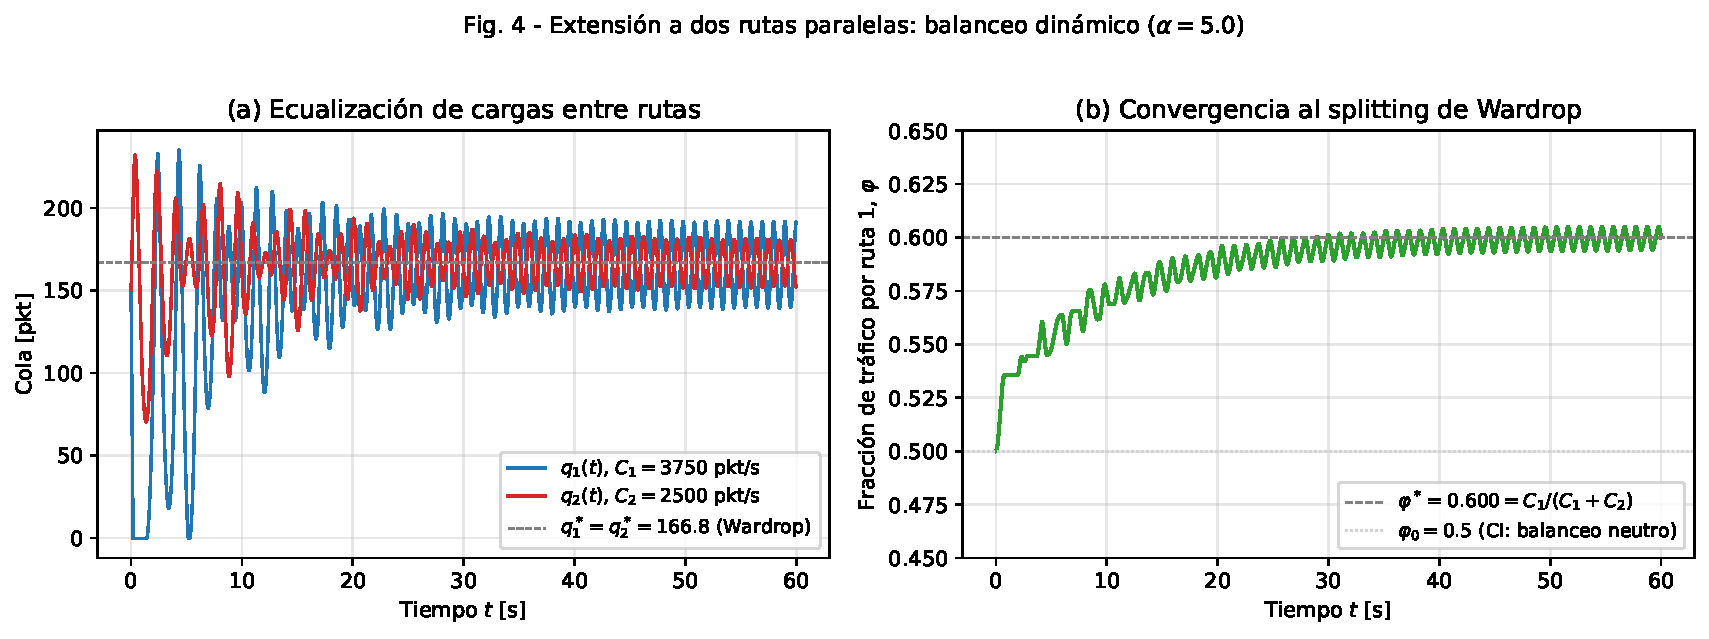
\includegraphics[width=\linewidth]{figs/fig4_routing.pdf}

\column{0.01\textwidth}

\column{0.45\textwidth}
\textbf{Pregunta de enrutamiento:} si hay dos rutas con capacidades distintas $C_1, C_2$, ¿cómo se reparte el tráfico?

\vspace{0.5em}
\textbf{Modelo extendido:} fracción $\varphi(t) \in [0,1]$ con dinámica de balanceo
$d\varphi/dt = -\alpha(p_1 - p_2)$.

\vspace{0.5em}
\textbf{Resultado:} converge al \emph{principio de Wardrop}: las pérdidas se igualan, $\varphi^* = C_1/(C_1+C_2)$.

\vspace{0.6em}
\small
\textit{Por límite de tiempo no profundizamos en esta extensión; está documentada en el repositorio.}

\vspace{0.3em}
\url{https://youtu.be/Q7I6CFJC0bc}
\end{columns}
\end{frame}

% --------- SLIDE 16: CONCLUSIONES ----------------------------------------
\begin{frame}{Conclusiones y aprendizajes}

\textbf{Lo que confirmamos:}
\begin{itemize}
\item Equilibrio analítico reproducido con error $< 0{,}02\%$.
\item Pendientes empíricas $1{,}04 / 3{,}76 / 4{,}10$
\item ABM4 supera a RK4 por factor $\sim 3$ en eficiencia.
\item Bifurcación de Hopf supercrítica en $w_q^c = 1{,}06 \times 10^{-2}$, con
amplitud $\sim \sqrt{w_q^c - w_q}$.
\end{itemize}

\vspace{0.5em}
\textbf{Lo que aprendimos al hacerlo:}
\begin{itemize}
\item Las discontinuidades de $p(x)$ degradan el orden empírico de los métodos de alto orden.
\item Euler tiene una cota de estabilidad $h < 2/|\lambda_{\max}|$ ineludible.
\item Análisis lineal y simulación no lineal coinciden cerca del equilibrio, divergen cuando la amplitud crece.
\end{itemize}

\vspace{0.4em}
\textbf{Extensiones naturales:} formulación con retardo (DDE), AQM modernos (PI, CoDel), topologías multi-cuello.
\end{frame}

% --------- SLIDE 17: GRACIAS ----------------------------------------------
\begin{frame}[standout]
Muchas gracias.

\small Espacio de preguntas

\vspace{1em}
\small\normalfont
\href{https://github.com/abel8000001/Proyecto-numerico}{\texttt{github.com/abel8000001/Proyecto-numerico}}
\end{frame}

\end{document}
